\documentclass[class=article,border=1pt]{standalone}
\usepackage{verbatim}
\usepackage{textcomp}
\usepackage{tikz}
\usetikzlibrary{shapes,arrows}
\usepackage[americaninductors,RPvoltages]{circuitikz}
\usepackage{amsmath}
\usepackage{pgfplots}
\pgfplotsset{compat=newest}

\begin{document}

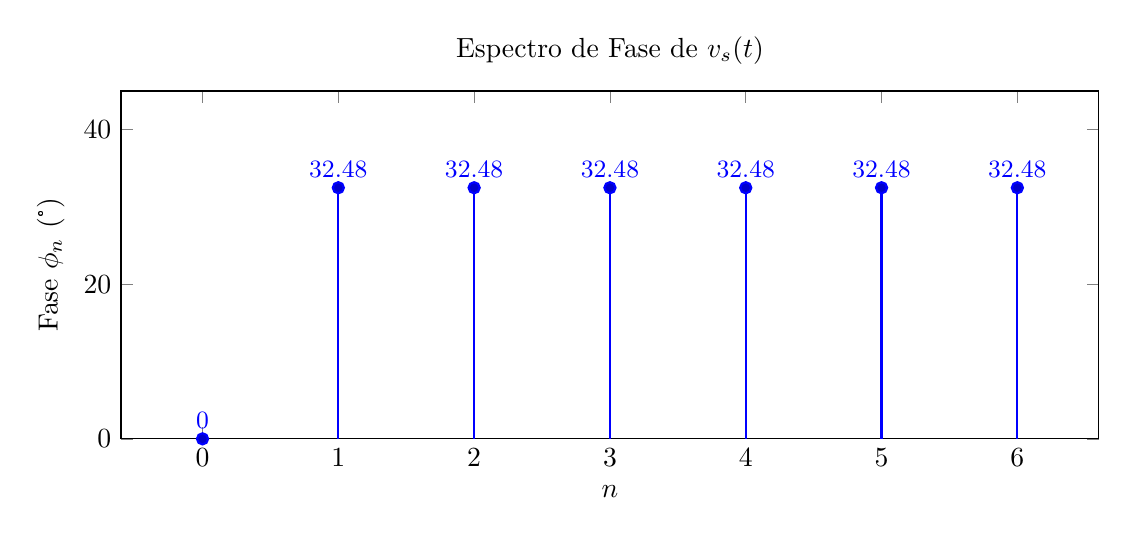
\begin{tikzpicture}
	\begin{axis}[
		title={Espectro de Fase de $v_s(t)$},
		xlabel={$n$},
		ylabel={Fase $\phi_n$ (°)},
		ymin=0, ymax=45,
		xtick={0,1,2,3,4,5,6},
		width=14cm,
		height=6cm,
		nodes near coords,
		every node near coord/.style={
			font=\small,
			anchor=south
		}
		]
		\addplot+[ycomb, thick, mark=*] coordinates {
			(0,0)
			(1,32.48)
			(2,32.48)
			(3,32.48)
			(4,32.48)
			(5,32.48)
			(6,32.48)
		};
	\end{axis}
\end{tikzpicture}

\end{document}
